\section{Discusión: Explicabilidad global y local}

\subsection{Explicabilidad global}

A nivel global, los tres modelos presentan distintos grados de transparencia y profundidad interpretativa, cada uno con fortalezas específicas según su estructura.

En el \textbf{árbol de decisión}, la explicabilidad global se manifiesta de forma visual y directa a través de las reglas. 
Su estructura jerárquica permite identificar con claridad las variables dominantes: la situación laboral, el número de antecedentes y la edad. 
El árbol ajustado consolida esta jerarquía en una forma fácilmente interpretable, situando la \textbf{condición de empleo} como nodo raíz y primera división crítica. 
Los individuos desempleados presentan una mayor probabilidad de reincidencia, mientras que una situación laboral estable se asocia con un menor riesgo, reflejando un patrón coherente con la literatura sobre reincidencia.

(\autoref{fig:tree_global_importances}).

\begin{figure}[h]
  \centering
  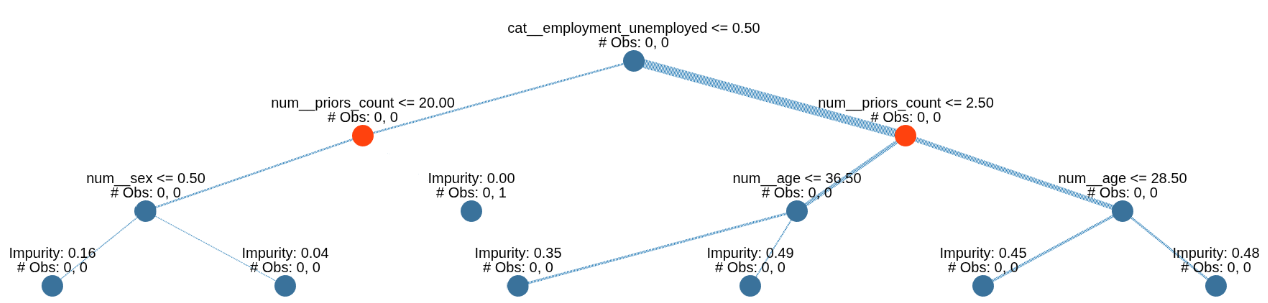
\includegraphics[width=0.85\linewidth]{figures/tree_global_importances.png}
  \caption{Importancia global de las variables en el árbol ajustado. 
  Se observa la predominancia de las variables relacionadas con el empleo, los antecedentes y la edad.}
  \label{fig:tree_global_importances}
\end{figure}

El \textbf{modelo logístico} mantiene una interpretabilidad transparente, pero desde un enfoque más cuantitativo. 
La magnitud y el signo de los coeficientes permiten medir la contribución exacta de cada variable: 
el desempleo y los antecedentes incrementan la probabilidad de reincidencia, mientras que el empleo y la edad actúan como factores protectores.
Esta relación se aprecia en la \autoref{fig:logistic_coefficients}, donde se muestra el impacto global de cada característica.

\begin{figure}[h]
  \centering
  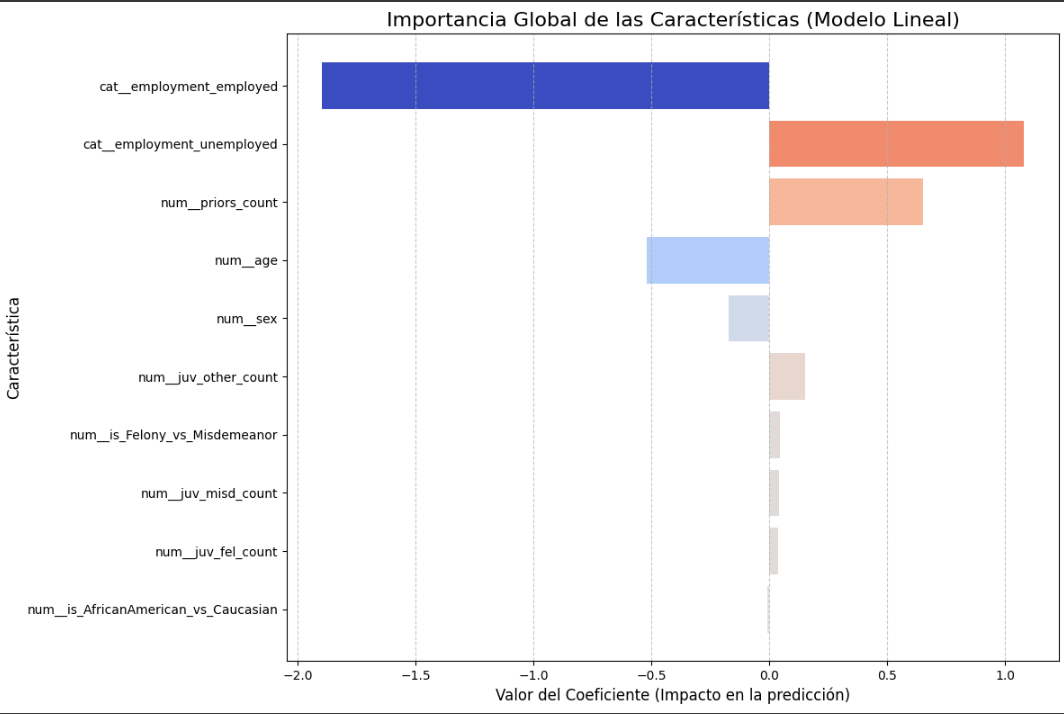
\includegraphics[width=0.85\linewidth]{figures/logistic_coefficients.png}
  \caption{Importancia global de las características en el modelo logístico. 
  Los coeficientes negativos (en azul) representan factores protectores frente a la reincidencia.}
  \label{fig:logistic_coefficients}
\end{figure}

Por su parte, el \textbf{GAM/EBM} se posiciona como el modelo con la explicabilidad más rica. 
A diferencia del árbol o del modelo lineal, el EBM permite observar el efecto de cada variable en forma de curvas de impacto, que reflejan transiciones suaves y umbrales de cambio. 
El empleo vuelve a ser la variable dominante, seguida de los antecedentes y la edad, confirmando las tendencias observadas en el análisis exploratorio. 
La \autoref{fig:ebm_global_effects} muestra la importancia global de cada término y las interacciones más relevantes detectadas.

\begin{figure}[h]
  \centering
  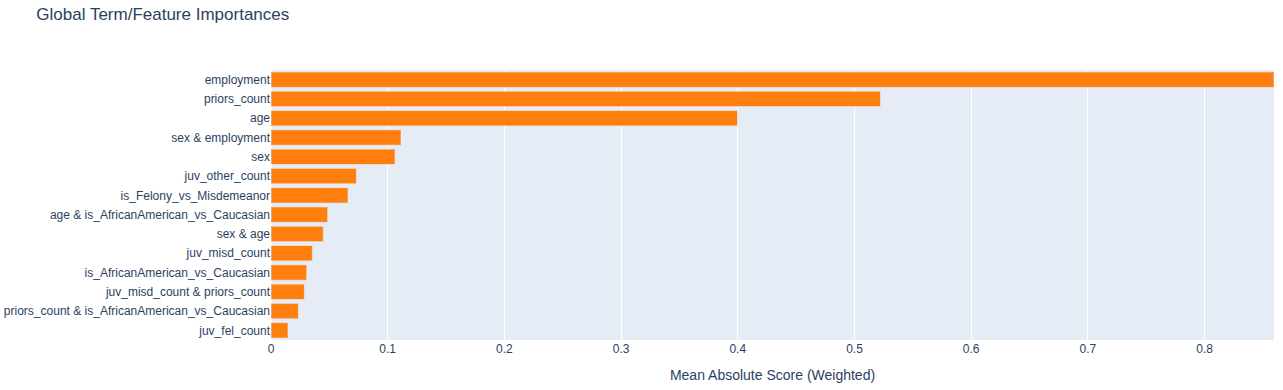
\includegraphics[width=\linewidth]{figures/ebm_global_effects.png}
  \caption{Importancia global de las características y términos en el modelo EBM. 
  Se observan los mayores pesos asociados al empleo, los antecedentes y la edad, junto a interacciones significativas como sexo–empleo.}
  \label{fig:ebm_global_effects}
\end{figure}

\subsection{Explicabilidad local}

A nivel local, los tres modelos permiten analizar cómo llegan a sus predicciones para casos individuales, pero lo hacen de formas muy distintas: el árbol mediante rutas de decisión explícitas, la regresión logística a través de pesos lineales y el EBM descomponiendo la predicción en contribuciones no lineales.

En el \textbf{árbol de decisión}, la explicación de una predicción individual se obtiene recorriendo los nodos hasta la hoja final. 
Cada condición define un punto de decisión que conduce a la clase final. 
La \autoref{fig:tree_local_example_caso_0} muestra un ejemplo real de esta lógica: el modelo predice reincidencia para un individuo desempleado, joven y con varios antecedentes. 
Las ramas coloreadas indican los nodos activos en la decisión y la intensidad del riesgo asociado a cada condición. 
Este tipo de representación facilita una lectura intuitiva y clara del razonamiento del modelo, aunque pierde precisión en escenarios con reglas más difusas o variables correlacionadas.

\begin{figure}[h]
  \centering
  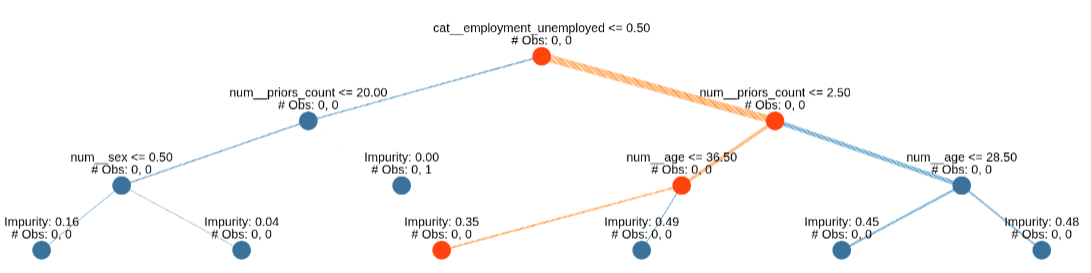
\includegraphics[width=0.9\linewidth]{figures/tree_local_example_caso_0.png}
  \caption{Explicabilidad local en el árbol de decisión. 
  Se observa la ruta de nodos que lleva a la predicción final (reincidencia), con las divisiones activas resaltadas en color.}
  \label{fig:tree_local_example_caso_0}
\end{figure}

En la \textbf{regresión logística}, la explicabilidad local se basa en la suma ponderada de los coeficientes globales. 
Cada variable contribuye de manera positiva o negativa al logit de salida, lo que permite entender cómo se acumulan los efectos individuales. 
En la \autoref{fig:logistic_local_contributions_caso_5}, correspondiente a un individuo con tres antecedentes, edad media y situación de desempleo, las barras naranjas reflejan los factores que incrementan la probabilidad de reincidencia, mientras que las azules indican efectos protectores. 
El modelo muestra un comportamiento coherente con su lógica global: el desempleo y los antecedentes dominan la decisión, mientras que la edad ejerce un efecto amortiguador. 

\begin{figure}[h]
  \centering
  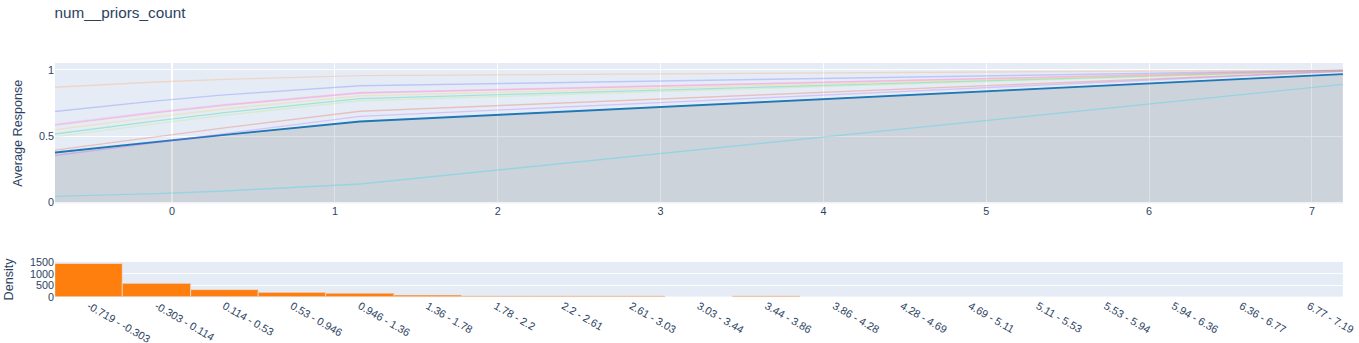
\includegraphics[width=0.85\linewidth]{figures/logistic_local_contributions_caso_5.png}
  \caption{Explicabilidad local del modelo logístico para un caso individual. 
  Las contribuciones positivas (naranja) aumentan la probabilidad de reincidencia, mientras que las negativas (azul) la reducen.}
  \label{fig:logistic_local_contributions_caso_5}
\end{figure}

El \textbf{modelo aditivo (GAM / EBM)} ofrece la explicabilidad local más rica y matizada. 
A diferencia del modelo lineal, las contribuciones de cada variable no son constantes, sino dependientes de su rango de valores. 
La \autoref{fig:ebm_local_explanations_caso_0} muestra un ejemplo donde el modelo predice reincidencia con una probabilidad del 65.6\%. 
El empleo (desempleado) y el número de antecedentes son los principales factores de riesgo, mientras que la edad actúa como un amortiguador parcial. 
Esta capacidad de modelar relaciones no lineales y explicarlas visualmente distingue al EBM como el modelo más transparente y completo a nivel local.

\begin{figure}[h]
  \centering
  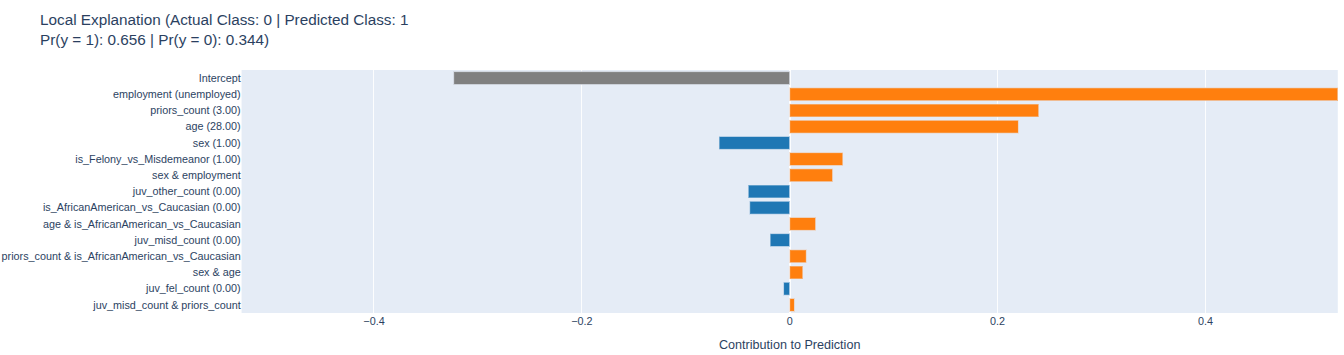
\includegraphics[width=0.9\linewidth]{figures/ebm_local_explanations_caso_0.png}
  \caption{Explicabilidad local del modelo EBM. 
  Cada barra representa el impacto de una variable en la predicción individual, con una descomposición no lineal que refleja tanto magnitud como dirección del efecto.}
  \label{fig:ebm_local_explanations_caso_0}
\end{figure}

\paragraph{Síntesis.}
En conjunto, los tres modelos presentan distintos niveles de granularidad en su capacidad explicativa:
el árbol destaca por su claridad lógica, la regresión logística por su coherencia estadística, y el EBM por su riqueza interpretativa y precisión local. 
Esta progresión evidencia cómo un incremento gradual en la complejidad del modelo puede mejorar la calidad de las explicaciones sin comprometer su transparencia.


\subsection{Comparativa general de interpretabilidad}

La comparación global y local entre los tres modelos muestra un gradiente claro de complejidad e interpretabilidad:

\begin{itemize}
  \item El \textbf{árbol de decisión} destaca por su \textbf{transparencia estructural}: es el modelo más fácil de entender, aunque menos flexible. Es ideal para justificar decisiones concretas o comunicar reglas de forma visual, pero sufre cierta pérdida de estabilidad cuando las relaciones entre variables son más sutiles.
  
  \item La \textbf{regresión logística} proporciona una \textbf{interpretabilidad cuantitativa y estable}, permitiendo medir la influencia de cada variable de manera directa a través de sus coeficientes. Sin embargo, su estructura estrictamente lineal le impide capturar bien las no linealidades o interacciones presentes en los datos. Es, por tanto, el modelo más “matemáticamente explicable”, aunque con menor capacidad de adaptación.
  
  \item El \textbf{GAM/EBM} combina ambas virtudes: mantiene una representación clara —basada en efectos univariantes y posibles interacciones— y logra la mejor precisión sin perder legibilidad. Su estructura modular permite analizar cada variable por separado, ofreciendo explicaciones globales mediante curvas de efecto y locales mediante contribuciones individuales. Esto lo convierte en el modelo más equilibrado entre precisión y transparencia.
\end{itemize}

En resumen, los tres enfoques demuestran que es posible alcanzar distintos equilibrios entre explicabilidad y rendimiento. 
El árbol ofrece comprensión inmediata, el modelo logístico aporta estabilidad y coherencia estadística, y el GAM/EBM integra flexibilidad y transparencia, consolidándose como la alternativa más completa del estudio en términos de interpretabilidad integral.

